\documentclass[a4paper,12pt,twoside]{memoir}

% Castellano
\usepackage[spanish,es-tabla]{babel}
\selectlanguage{spanish}
\usepackage[utf8]{inputenc}
\usepackage[T1]{fontenc}
\usepackage{lmodern} % Scalable font
\usepackage{microtype}
\usepackage{placeins}
\usepackage{textgreek} % letras griegas

\RequirePackage{booktabs}
\RequirePackage[table]{xcolor}
\RequirePackage{xtab}
\RequirePackage{multirow}

% Links
\PassOptionsToPackage{hyphens}{url}\usepackage[colorlinks]{hyperref}
\hypersetup{
	allcolors = {red}
}

% Ecuaciones
\usepackage{amsmath}

% Rutas de fichero / paquete
\newcommand{\ruta}[1]{{\sffamily #1}}

% Párrafos
\nonzeroparskip

% Huérfanas y viudas
\widowpenalty100000
\clubpenalty100000

% Imagenes
\usepackage{graphicx}
\newcommand{\imagen}[2]{
	\begin{figure}[!h]
		\centering
		\includegraphics[width=0.9\textwidth]{#1}
		\caption{#2}\label{fig:#1}
	\end{figure}
	\FloatBarrier
}

\newcommand{\imagenflotante}[2]{
	\begin{figure}%[!h]
		\centering
		\includegraphics[width=0.9\textwidth]{#1}
		\caption{#2}\label{fig:#1}
	\end{figure}
}



% El comando \figura nos permite insertar figuras comodamente, y utilizando
% siempre el mismo formato. Los parametros son:
% 1 -> Porcentaje del ancho de página que ocupará la figura (de 0 a 1)
% 2 --> Fichero de la imagen
% 3 --> Texto a pie de imagen
% 4 --> Etiqueta (label) para referencias
% 5 --> Opciones que queramos pasarle al \includegraphics
% 6 --> Opciones de posicionamiento a pasarle a \begin{figure}
\newcommand{\figuraConPosicion}[6]{%
  \setlength{\anchoFloat}{#1\textwidth}%
  \addtolength{\anchoFloat}{-4\fboxsep}%
  \setlength{\anchoFigura}{\anchoFloat}%
  \begin{figure}[#6]
    \begin{center}%
      \Ovalbox{%
        \begin{minipage}{\anchoFloat}%
          \begin{center}%
            \includegraphics[width=\anchoFigura,#5]{#2}%
            \caption{#3}%
            \label{#4}%
          \end{center}%
        \end{minipage}
      }%
    \end{center}%
  \end{figure}%
}

%
% Comando para incluir imágenes en formato apaisado (sin marco).
\newcommand{\figuraApaisadaSinMarco}[5]{%
  \begin{figure}%
    \begin{center}%
    \includegraphics[angle=90,height=#1\textheight,#5]{#2}%
    \caption{#3}%
    \label{#4}%
    \end{center}%
  \end{figure}%
}
% Para las tablas
\newcommand{\otoprule}{\midrule [\heavyrulewidth]}
%
% Nuevo comando para tablas pequeñas (menos de una página).
\newcommand{\tablaSmall}[5]{%
 \begin{table}
  \begin{center}
   \rowcolors {2}{gray!35}{}
   \begin{tabular}{#2}
    \toprule
    #4
    \otoprule
    #5
    \bottomrule
   \end{tabular}
   \caption{#1}
   \label{tabla:#3}
  \end{center}
 \end{table}
}

%
% Nuevo comando para tablas pequeñas (menos de una página).
\newcommand{\tablaSmallSinColores}[5]{%
 \begin{table}[H]
  \begin{center}
   \begin{tabular}{#2}
    \toprule
    #4
    \otoprule
    #5
    \bottomrule
   \end{tabular}
   \caption{#1}
   \label{tabla:#3}
  \end{center}
 \end{table}
}

\newcommand{\tablaApaisadaSmall}[5]{%
\begin{landscape}
  \begin{table}
   \begin{center}
    \rowcolors {2}{gray!35}{}
    \begin{tabular}{#2}
     \toprule
     #4
     \otoprule
     #5
     \bottomrule
    \end{tabular}
    \caption{#1}
    \label{tabla:#3}
   \end{center}
  \end{table}
\end{landscape}
}

%
% Nuevo comando para tablas grandes con cabecera y filas alternas coloreadas en gris.
\newcommand{\tabla}[6]{%
  \begin{center}
    \tablefirsthead{
      \toprule
      #5
      \otoprule
    }
    \tablehead{
      \multicolumn{#3}{l}{\small\sl continúa desde la página anterior}\\
      \toprule
      #5
      \otoprule
    }
    \tabletail{
      \hline
      \multicolumn{#3}{r}{\small\sl continúa en la página siguiente}\\
    }
    \tablelasttail{
      \hline
    }
    \bottomcaption{#1}
    \rowcolors {2}{gray!35}{}
    \begin{xtabular}{#2}
      #6
      \bottomrule
    \end{xtabular}
    \label{tabla:#4}
  \end{center}
}

%
% Nuevo comando para tablas grandes con cabecera.
\newcommand{\tablaSinColores}[6]{%
  \begin{center}
    \tablefirsthead{
      \toprule
      #5
      \otoprule
    }
    \tablehead{
      \multicolumn{#3}{l}{\small\sl continúa desde la página anterior}\\
      \toprule
      #5
      \otoprule
    }
    \tabletail{
      \hline
      \multicolumn{#3}{r}{\small\sl continúa en la página siguiente}\\
    }
    \tablelasttail{
      \hline
    }
    \bottomcaption{#1}
    \begin{xtabular}{#2}
      #6
      \bottomrule
    \end{xtabular}
    \label{tabla:#4}
  \end{center}
}

%
% Nuevo comando para tablas grandes sin cabecera.
\newcommand{\tablaSinCabecera}[5]{%
  \begin{center}
    \tablefirsthead{
      \toprule
    }
    \tablehead{
      \multicolumn{#3}{l}{\small\sl continúa desde la página anterior}\\
      \hline
    }
    \tabletail{
      \hline
      \multicolumn{#3}{r}{\small\sl continúa en la página siguiente}\\
    }
    \tablelasttail{
      \hline
    }
    \bottomcaption{#1}
  \begin{xtabular}{#2}
    #5
   \bottomrule
  \end{xtabular}
  \label{tabla:#4}
  \end{center}
}



\definecolor{cgoLight}{HTML}{EEEEEE}
\definecolor{cgoExtralight}{HTML}{FFFFFF}

%
% Nuevo comando para tablas grandes sin cabecera.
\newcommand{\tablaSinCabeceraConBandas}[5]{%
  \begin{center}
    \tablefirsthead{
      \toprule
    }
    \tablehead{
      \multicolumn{#3}{l}{\small\sl continúa desde la página anterior}\\
      \hline
    }
    \tabletail{
      \hline
      \multicolumn{#3}{r}{\small\sl continúa en la página siguiente}\\
    }
    \tablelasttail{
      \hline
    }
    \bottomcaption{#1}
    \rowcolors[]{1}{cgoExtralight}{cgoLight}

  \begin{xtabular}{#2}
    #5
   \bottomrule
  \end{xtabular}
  \label{tabla:#4}
  \end{center}
}



\graphicspath{ {./img/} }

% Capítulos
\chapterstyle{bianchi}
\newcommand{\capitulo}[2]{
	\setcounter{chapter}{#1}
	\setcounter{section}{0}
	\setcounter{figure}{0}
	\setcounter{table}{0}
	\chapter*{#2}
	\addcontentsline{toc}{chapter}{#2}
	\markboth{#2}{#2}
}

% Apéndices
\renewcommand{\appendixname}{Apéndice}
\renewcommand*\cftappendixname{\appendixname}

\newcommand{\apendice}[1]{
	%\renewcommand{\thechapter}{A}
	\chapter{#1}
}

\renewcommand*\cftappendixname{\appendixname\ }

% Formato de portada
\makeatletter
\usepackage{xcolor}
\newcommand{\tutor}[1]{\def\@tutor{#1}}
\newcommand{\course}[1]{\def\@course{#1}}
\definecolor{cpardoBox}{HTML}{E6E6FF}
\def\maketitle{
  \null
  \thispagestyle{empty}
  % Cabecera ----------------
\noindent
\includegraphics[width=\textwidth]{cabecera}\vspace{1cm}%
  \vfill
  % Título proyecto y escudo informática ----------------
  \colorbox{cpardoBox}{%
    \begin{minipage}{.8\textwidth}
      \vspace{.5cm}\Large
      \begin{center}
      \textbf{TFG del Grado en Ingeniería Informática}\vspace{.6cm}\\
      \textbf{\LARGE\@title{}}
      \end{center}
      \vspace{.2cm}
    \end{minipage}

  }%
  \hfill\begin{minipage}{.20\textwidth}
    
\includegraphics[width=\textwidth]{escudoInfor}
  \end{minipage}
  \vfill
  % Datos de alumno, curso y tutores ------------------
  \begin{center}%
  {%
    \noindent\LARGE
    Presentado por \@author{}\\ 
    en Universidad de Burgos --- \@date{}\\
    Tutores: \@tutor{}\\
    
    
  }%
  \end{center}%
  \null
  \cleardoublepage
  }
\makeatother

\newcommand{\nombre}{Humberto Marijuán Santamaría} %%% cambio de comando

% Datos de portada
\title{Modelos de Mezcla}
\author{\nombre}
\tutor{Luis R. Izquierdo y José Manuel Galán}
\date{\today}

\begin{document}

\maketitle


\newpage\null\thispagestyle{empty}\newpage


%%%%%%%%%%%%%%%%%%%%%%%%%%%%%%%%%%%%%%%%%%%%%%%%%%%%%%%%%%%%%%%%%%%%%%%%%%%%%%%%%%%%%%%%
\thispagestyle{empty}


\noindent
\includegraphics[width=\textwidth]{cabecera}\vspace{1cm}

\noindent D. Luis R. Izquierdo y D. José Manuel Galán, profesores del departamento Ingeniería de Organización, área de Organización de Empresas.

\noindent Expone:

\noindent Que el alumno D. \nombre, con DNI 71757204X, ha realizado el Trabajo final de Grado en Ingeniería Informática titulado Modelos de Mezcla. 

\noindent Y que dicho trabajo ha sido realizado por el alumno bajo la dirección del que suscribe, en virtud de lo cual se autoriza su presentación y defensa.

\begin{center} %\large
En Burgos, {\large \today}
\end{center}

\vfill\vfill\vfill

% Author and supervisor
\begin{minipage}{0.45\textwidth}
\begin{flushleft} %\large
Vº. Bº. del Tutor:\\

\includegraphics[width=0.8\textwidth]{img/firma-luis-transparente}\\[0.3cm]
D. Luis R. Izquierdo
\end{flushleft}
\end{minipage}
\hfill
\begin{minipage}{0.45\textwidth}
\begin{flushleft} %\large
Vº. Bº. del co-tutor:\\

\includegraphics[width=0.7\textwidth]{img/Firma_Transparente}\\
D. José Manuel Galán 
\end{flushleft}
\end{minipage}
\hfill

\vfill

% para casos con solo un tutor comentar lo anterior
% y descomentar lo siguiente
%Vº. Bº. del Tutor:\\[2cm]
%D. nombre tutor


\newpage\null\thispagestyle{empty}\newpage




\frontmatter

% Abstract en castellano
\renewcommand*\abstractname{Resumen}
\begin{abstract}
En este documento se expone el proceso de desarrollo de una herramienta de cálculos estadísticos sobre \emph{Mixing Models} (modelos de mezcla). Este tipo de herramientas suelen resolver problemas en el ámbito de la ecología, permitiendo calcular las contribuciones de diferentes fuentes a una determinada mezcla a partir de trazadores. Algunos ejemplos de aplicaciones son el cálculo de la dieta de un animal a partir de la composición de sus sus heces, o la estimación de la procedencia geográfica de diferentes tipos de tierra que componen un sedimento. 

Se ha creado una aplicación web que utiliza las librería GLPK para resolver problemas de maximización y minimización por medio de una interfaz en \emph{Typescript}. Esta aplicación web permite visualizar y exportar los resultados. El código de la aplicación web esta desarrollado en \emph{Angular} y utiliza otros lenguajes habituales en las aplicaciones web como HTML y CSS. La aplicación esta internacionalizada a los idiomas Español e Inglés.

La aplicación permite la carga de datos a partir de archivos .csv e incluye un vídeo tutorial como guía de uso. Por último se realizó el despliegue del proyecto en Netlify con url: \url{https://mixingmodels.netlify.app}
\end{abstract}

\renewcommand*\abstractname{Descriptores}
\begin{abstract}
Aplicación web, single-page aplication, composición dieta, ecuaciones lineales con restricciones.
\end{abstract}

\clearpage

% Abstract en inglés
\renewcommand*\abstractname{Abstract}
\begin{abstract}
This document presents the development process of a statistical calculation tool based on so-called \emph{Mixing Models}. This type of tool is often used to solve problems in the field of ecology, allowing to calculate the contributions of different sources to a certain mixture using tracers. 

A web application has been created that uses the GLPK library to solve maximisation and minimisation problems by means of a Typescript interface, allowing the results to be visualised and exported. The code of the web application has been developed in \emph{Angular} and uses other common languages in web applications such as HTML and CSS. The application is internationalised in Spanish and English.

The application allows the loading of data from .csv files and includes a video tutorial as a user guide. Finally, the project was deployed in Netlify with url: \url{https://mixingmodels.netlify.app}
\end{abstract}

\renewcommand*\abstractname{Keywords}
\begin{abstract}
Web application, single-page application, diet composition, linear equations with constraints.
\end{abstract}

\clearpage

% Indices
\tableofcontents

\clearpage

\listoffigures

\clearpage

\listoftables
\clearpage

\mainmatter
\capitulo{1}{Introducción}

Este proyecto comienza con la necesidad de crear una aplicación web que permita estimar diferencias y composición de la dieta de vertebrados herbívoros. Este problema está definido en el artículo: \emph{''Using n-alkanes to estimate diet composition of herbivores: a novel mathematical approach''} \cite{problemn-alkanes2007} en el cual se plantea la resolución de un sistema de ecuaciones con restricciones, con el objetivo de calcular la composición de la dieta de diferentes especies de herbívoros. Este problema pretende responder a la pregunta de ¿Cuáles son las proporciones máximas y mínimas de cada componente de la dieta?.

Los modelos de mezcla son utilizados para estimar contribuciones de diferentes fuentes a una mezcla. Estos modelos suelen requerir datos que actúan como marcadores que caractericen rasgos (comúnmente químicos) de las fuentes y las mezclas. Los modelos de mezcla están muy presentes en el ámbito de  la ecología, utilizando isótopos estables como trazadores para evaluar la contribución de los componentes de la dieta (fuentes) a la dieta de los consumidores (mezcla). Aunque este problema tiene otras muchas aplicaciones: movimiento de animales, origen de los contaminantes, transferencia de nutrientes entre ecosistemas, huellas de la erosión de los sedimentos y evaluar las relaciones entre depredadores y presas desde perfiles de ácidos grasos \cite{bicknell:2014,bartov:2012,granek:2009,blake:2012,neubauer:2015}.

En este trabajo de fin de grado, se ha diseñado una aplicación web que permite resolver sistemas de ecuaciones con restricciones, para lo cual se ha hecho uso de algunas librerías \emph{open source} que han facilitado la resolución del problema (librería GLPK \cite{glpk:package} y algunos paquetes Node). 

\section{Estructura de la memoria}

La estructura de este documento viene formada por siete capítulos:

\begin{itemize}
    \item \textbf{1. Introducción:} Una descripción breve del marco donde se encuentra. Y la estructura de la memoria y los anexos.
    \item \textbf{2. Objetivos del proyecto:} hemos definido los requisitos de este proyecto, distinguiendo entre generales, funcionales y técnicos.
    \item \textbf{3. Conceptos teóricos:} Exposición conocimientos para facilitar la compresión del proyecto.
    \item \textbf{4. Técnicas y herramientas:} Listado de metodologías y herramientas utilizadas en el proyecto
    \item \textbf{5. Aspectos relevantes del desarrollo del proyecto:} Se ha resumido el proceso de desarrollo del proyecto, destacando aspectos claves del mismo.
    \item \textbf{6. Trabajos relacionados:} Se ha realizado una búsqueda de trabajos similares al software presentado.
    \item \textbf{7. Conclusiones y Líneas de trabajo futuras:} Conclusión personal del proyecto y posibles vías de trabajo futuras.
\end{itemize}

\section{Estructura de los anexos}

\begin{itemize}
    \item \textbf{Plan de Proyecto Software:} Planificación temporal y estudio de viabilidad económica y legal.
    \item \textbf{Especificación de Requisitos:} Objetivos y requisitos iniciales del proyecto.
    \item \textbf{Especificación de diseño:} Recoge lo referente al diseño de la aplicación, incluyendo diseño de datos, procedimental y arquitectónico.
    \item \textbf{Documentación técnica de programación:} Explica la estructura de los directorios del repositorio GitHub, junto con manuales orientados al programador (instalación, compilación y ejecución del proyecto).
    \item \textbf{Documentación de usuario:} Es una guía de uso de la aplicación paso por paso con capturas de la interfaz.
\end{itemize}
\capitulo{2}{Objetivos del proyecto}

En este apartado se definen los requisitos del proyecto distinguiendo entre objetivos generales, requisitos de software y objetivos técnicos.

\section{Objetivos generales}

El objetivo principal de este proyecto es implementar una aplicación web que resuelva problemas de programación lineal dentro del contexto de \emph{Mixing models} (modelos de mezcla). Esta aplicación deberá ser accesible desde cualquier sistema operativo y móvil. La aplicación web se  implementará como una Single-page application. La vista de la interfaz deberá ser simple e intuitiva.

\section{Objetivos de funcionalidad}

\begin{itemize}
    \item \textbf{Usabilidad y diseño:} La aplicación web debe ser fácil de usar para el usuario, y fácil de entender para los usuarios que estén familiarizados con el problema.
    \item \textbf{Accesibilidad:} La web debe ser accesible por la mayor parte de navegadores en los principales sistemas operativos.
    \item \textbf{Importación y Exportación:} Se debe permitir la descarga de las soluciones y la importación de los datos del problema. %Con el objetivo de aportar una mayor agilidad en el manejo de la aplicación.
    \item \textbf{Internacionalización:} La aplicación debe incorporar todos los textos tanto en Español como en Inglés. Asimismo, deberá permitir la incorporación de idiomas adicionales sin que esto conlleve a realizar cambios en el código.
\end{itemize}

\section{Objetivos técnicos}

\begin{itemize}
    \item Utilización de la metodología Scrum para el seguimiento y el control del proyecto, siendo necesario trabajar con herramientas de gestión de proyectos y de control de versiones durante el desarrollo.
    \item Selección y aprendizaje de un lenguaje de programación para desarrollar una aplicación web .
	\item Creación de una aplicación web que realice  peticiones web a una API .
	\item Generación de ficheros .csv a partir de los  datos resultantes. Exportaciones de los cálculos intermedios, de la solución  junto con los datos del problema y un último documento que tenga la estructura permitida en la carga de datos. La visualización de los informes debe ser similar a visual de  la aplicación web.
	\item Carga de datos por medio de ficheros .csv.
	\item Utilización de librerías para resolver problemas de programación lineal.
	\item La aplicación deberá contener un apartado de guía, que tendrá que ser accesible desde la aplicación en cualquier momento.
	\item Interfaz gráfica simple y limpia.
    \item Utilización de herramientas de análisis de código.
\end{itemize}
\capitulo{3}{Conceptos teóricos}

En este capitulo se han recogido algunos conocimientos básicos sobre los \emph{Mixing Models} que son necesarios para enmarcar el problema. Además tenemos como objetivo explicar el problema que se resuelve con la aplicación.

\section{Mixing Models}

Los modelos de mezcla (\emph{Mixing Models}) son herramientas estadísticas que utilizan biotrazadores para estimar las contribuciones de diversas fuentes a una mezcla.
Estas herramientas son usadas en muchos problemas. A continuación se expondrán algunos ejemplos donde se usan los \emph{Mixing Models}:

%\clearpage

\subsection{La dieta en la ecología}

La dieta en ecología  (fuentes = presas, mezcla = dieta de un consumidor). En el ejemplo de la Figura \ref{fig:preyDiet} se usan los \emph{Mixing Models} para calcular las contribuciones de diferentes presas del entorno (p. ej. mamíferos marinos, salmones, ciervos) a la dieta de un depredador (p. ej. Lobo) a partir de la composición de sus heces. En el artículo \cite{improveBayes2009} se resuelve este problema usando MixSir y se obtuvieron resultados robustos. Por último, Jackson et al. (2009) \cite{improveBayes2009} propone añadir parámetros de error adicionales al ámbito de la mezcla .

\begin{figure}[h!] 
\centering
    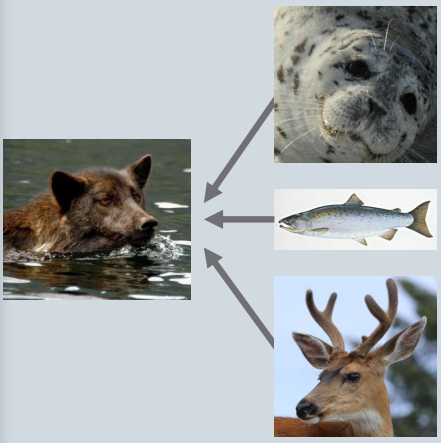
\includegraphics[width=0.8\textwidth]{img/preyDiet.PNG}
\caption{Ejemplo dieta en ecología }
\label{fig:preyDiet}
\end{figure}

\clearpage

\subsection{Movimiento en ecología}

Los modelos de mezcla también se utilizan en ecología para estimar movimientos de animales (fuentes = regiones, mezcla =  animales que pueden desplazarse entre regiones). Estos modelos son usados por ecologistas para calcular composiciones de comunidades y la biodiversidad a nivel de sitio terrestre de todo el mundo.

Para más información artículo \emph{``The PREDICTS database: a global database of how local terrestrial biodiversity responds to human impacts''} \cite{biodiversity:2014}.

\begin{figure}[h!] 
\centering
    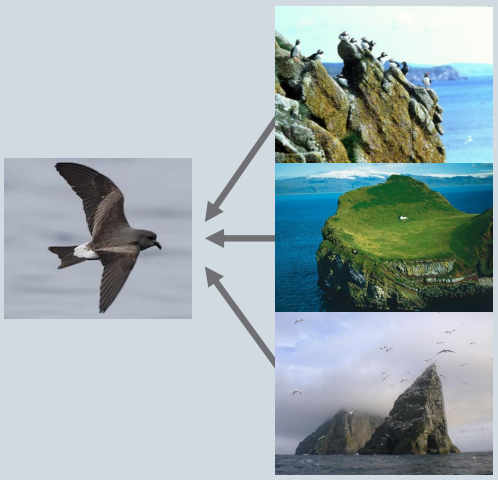
\includegraphics[width=0.8\textwidth]{img/colonyBird.PNG}
\caption{Ejemplo Movimiento en ecología }
\label{fig:colonyBird}
\end{figure}

\clearpage

\subsection{Sedimentos en sistemas fluviales}

Sedimentos en sistemas fluviales (fuentes = terrenos aguas arriba, mezcla = sedimentos aguas abajo). El objetivo de los sistemas de agricultura regenerativa \cite{rodale:1983} es aumentar la calidad del suelo y la biodiversidad de las tierras de labranza, favoreciendo la creación de productos agrícolas nutritivos de forma rentable.

%TODO: \url{https://peerj.com/articles/4428/}
artículo: \url{https://pubmed.ncbi.nlm.nih.gov/30812003/}

\begin{figure}[h!] 
\centering
    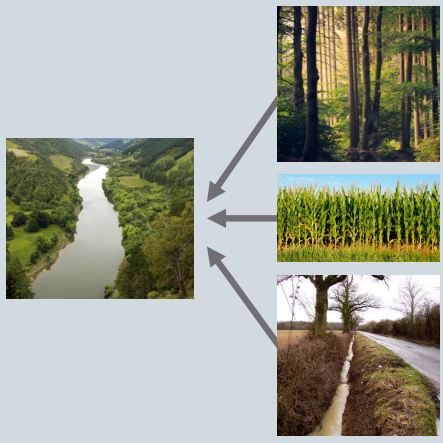
\includegraphics[width=0.8\textwidth]{img/soilSediment.PNG}
\caption{Ejemplo Sedimentos en sistemas fluviales }
\label{fig:soilSediment}
\end{figure}


\clearpage

\section{Cómo funcionan los \emph{Mixing Models}}

Comenzamos explicando un problema sencillo. El problema se plantea dadas dos fuentes posibles de alimentos (Source 1, Source 2) y un consumidor (ver fig. \ref{fig:workMixing0}). Nuestro objetivo es identificar la dieta del consumidor a partir de la composición de sus heces. Para ello, se hace uso de biotrazadores o marcadores, que se encuentran presentes en las fuentes y no se alteran en el proceso de digestión. De esta forma, los biotrazadores nos permiten realizar estimaciones de la cantidad de cada una de las fuentes que puede haber ingerido un consumidor. 

\begin{figure}[h!] 
\centering
    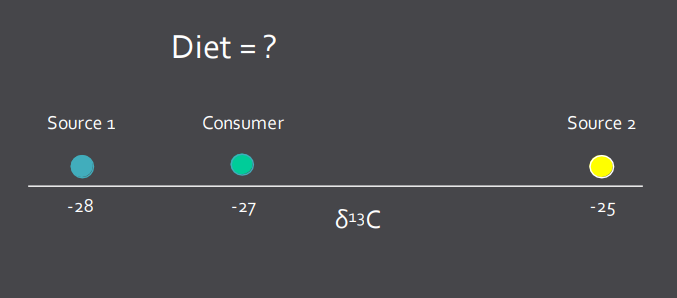
\includegraphics[width=0.8\textwidth]{img/workMixing0.PNG}
\caption{Linear \emph{Mixing Models} - Problema }
\label{fig:workMixing0}
\end{figure}

Para simplificar la explicación supondremos que la masa se conserva durante el proceso de digestión, por ello partimos de la ecuación $p_1 + p_2 = 1$, donde $p_i$ denota la masa de fuente (\emph{source}) $i$ por cada unidad de masa de heces. Como suponemos que la masa se conerva, la suma de las proporciones de las fuentes es igual a 1. Tenemos también una segunda ecuación que refleja la conservación de la masa del biotrazador \textdelta$_{13}C$ a través del proceso de digestión: $Consumer = p_1*S_1 + p_2*S_2$, donde $Consumer$ es la masa de biotrazador en las heces, y $S_i$ denota la concentración de biotrazador en la fuente $i$.

\begin{figure}[h!] 
\centering
    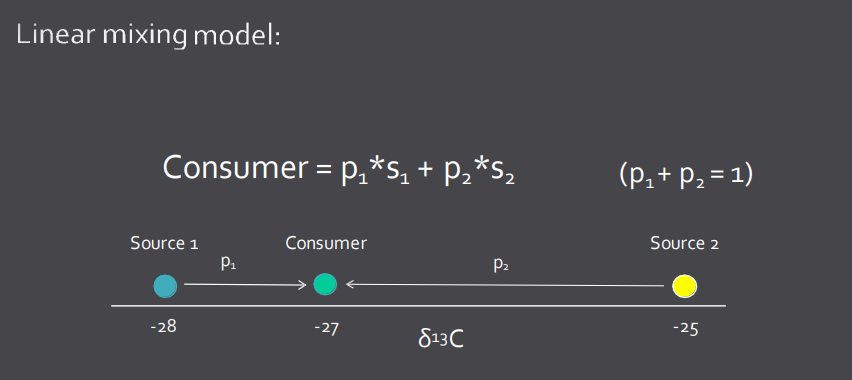
\includegraphics[width=0.8\textwidth]{img/workMixing1.PNG}
\caption{Linear \emph{Mixing Models} - Ecuaciones con un marcador }
\label{fig:workMixing1}
\end{figure}

En el caso de la figura \ref{fig:workMixing1} solo teníamos un eje / biotrazador / marcador, por lo que solo considerábamos una ecuación. En el figura \ref{fig:workMixing2} tenemos dos ejes para los biotrazadores: \textdelta$_{13}C$ y \textdelta$_{15}N$, además de una fuente más ($S_1$, $S_2$, $S_3$). En consecuencia, podemos usar las siguientes ecuaciones: 

$$ Consumer_C = p_1*S_{1C} + p_2*S_{2C} + p_3*S_{3C} $$
$$ Consumer_N = p_1*S_{1N} + p_2*S_{2N} + p_3*S_{3N} $$
$$ p_1 + p_2 = 1 $$

Siendo $S_{iN}$ la concentración del segundo biotrazador  (\textdelta$_{15}N$) en la fuente $i$,  y ese valor se multiplicara por la proporción de la fuente $i$ que se ha ingerido.

\begin{figure}[h!] 
\centering
    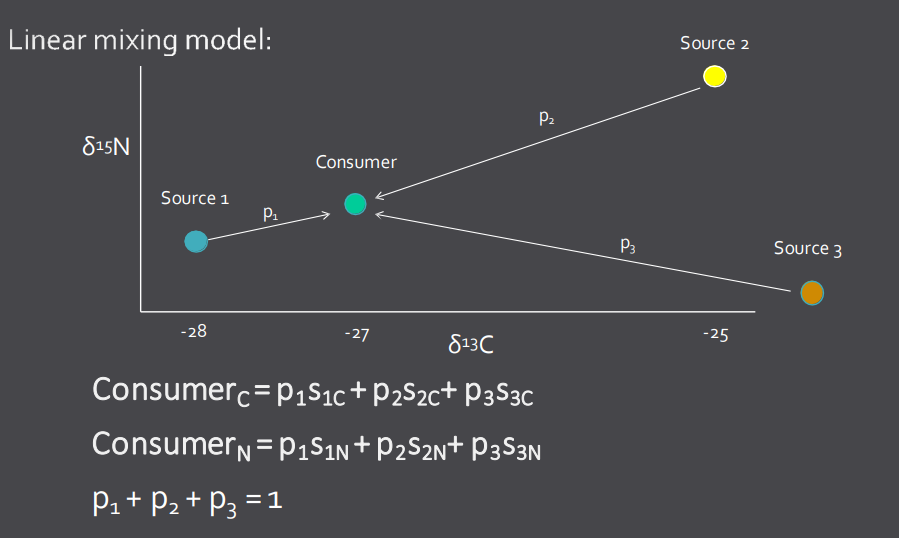
\includegraphics[width=0.8\textwidth]{img/workMixing2.PNG}
\caption{Linear \emph{Mixing Models} - Ecuaciones con dos marcadores }
\label{fig:workMixing2}
\end{figure}

%\subsection{}

En el caso de mi aplicación, se diseñó sin imponer la condición de conservación de la masa. Esto ha ofrecido un mayor realismo a los cálculos de la aplicación, ya que en general la masa de las heces no coincide necesariamente con la suma de las masas que se ingieren (p. ej. los alimentos ingeridos suelen tener más concentración de agua que las heces).

\newpage
\section{Problema n-alcanos}

En esta sección hemos resumido el problema planteado en el artículo \emph{``Using n-alkanes to estimate diet composition of herbivores: a novel mathematical approach''} \cite{problemn-alkanes2007}, que es el punto de partida del proyecto.

Los n-alcanos son hidrocarburos que se encuentran en las cutículas de las plantas, y que pueden ser usados para estimar la composición de la dieta de herbívoros a partir de la composición de sus heces. Conocer la composición de la dieta de los herbívoros es importante para comprender su ecología y alimentación, lo cual es útil para medir sus efectos sobre la vegetación y los ecosistemas.

El modelo usa programación lineal para estimar el mínimo y el máximo de las proporciones de cada planta de la dieta.

Las especies de plantas se caracterizan por diferentes concentraciones de n-alcanos. Los marcadores químicos recuperados en las heces pueden ser utilizados para cuantificar las plantas ingeridas por un animal.
	
Supongamos que $d$ es el número de n-alcanos en planta y hez. Cada hez de la muestra puede ser considerada un \textbf{punto} en el espacio d-Euclideo, que describe la concentración de cada uno de los d n-alcanos. Cada especie de planta puede ser interpretada como un vector en este espacio (Figura \ref{fig:espacio01}).

\begin{figure}[h!] 
\centering
    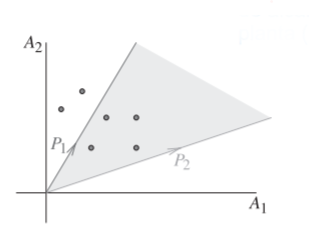
\includegraphics[width=0.4\textwidth]{img/espacio01.png}
\caption{Representación de dos alcanos ($A_1$,$A_2$), dos especies de plantas (vectores $P_1$ y $P_2$), y seis muestras de heces (puntos de la figura). El área sombreada es el cono bidimensional generado por los vectores $P_1$ y $P_2$.}
\label{fig:espacio01}
\end{figure}

Las dietas son combinaciones lineales, es decir, las sumas ponderadas de los vectores que representan las especies vegetales. El peso o coeficiente de cada vector define la cantidad correspondiente de la especie en la dieta. Cada coeficiente dividido  por el sumatorio de los coeficientes, da la proporción de cada planta en la dieta. Si $P_1, P_2, ..., P_p$ son los d-vectores que representan p plantas, cada vector indica la concentración de n-alcanos en esa especie, la combinación lineal con coeficientes $c_1,c_2, ... , c_p$ es $c_1 P_1 + c_2 P_2 + ... + c_p P_p$. \\
Las combinaciones lineales con coeficientes negativos son \textit{"dietas sin sentido"}. Por lo tanto, debemos centrar nuestra atención en las combinaciones lineales que tienen coeficientes no negativos. Este conjunto de combinaciones lineales no negativas forma el cono generado por esos dos vectores. En la Figura \ref{fig:espacio01} el cono generado por los vectores $P_1$ y $P_2$ es la región sombreada. Usamos $C$ para denotar el cono generado, es decir: $$ C = { c_1 P_1 + c_2 P_2 + ... + c_p P_p, \text{ con } c_1,c_2,...,c_p >=0} $$

La estimación de dietas a partir de pruebas fecales $F_1, F_2, ... . F_q $ toma una muestra $F$ y busca sí:

\begin{enumerate}[(i)]
\item $F$ pertenece al cono $C$ o
\item $F$ es un punto fuera de $C$.
\end{enumerate}

Esto es determinado resolviendo el sistema de ecuaciones linear $$Ax=F.$$

Donde A es una matriz $d \times p$ cuyas columnas son los vectores $P_1, P_2 , ... , P_p$ que representan las plantas. Si todos los componentes de la solución $x$ son no-negativos, estaremos en el caso $_{(I)}$, y $x$ especifica la composición correspondiente de especies en las heces. Si hay un componente negativo, estamos en la situación $_{(II)}$, indicando que son \textit{"dietas sin sentido"}. Esto puede resultar de errores en la medición de las concentraciones de n-alcanos, o la existencia de plantas no incluidas en la muestra. Una posible solución es encontrar un vector no negativo de coeficientes que se aproximen a la $x$. Un posible enfoque consiste en:

\begin{enumerate}[(i)]
\setcounter{enumi}{2}
\item identificar un punto $F_0$ en el cono $C$ considerado \textit{"similar a"} $F$, y
\item usando $F_0$ en lugar de $F$, proceder resolviendo como en $_{(I)}$ el sistema de ecuaciones.
\end{enumerate}

Normalmente, la proyección de $F$ en $C$, es decir, el punto en $C$ más cercano a $F$, es seleccionado para ser $F_0$. En la figura \ref{fig:espacio01} hay dos puntos en el caso $_{(II)}$. Cada uno será remplazado por su proyección en $C$, por lo que se encontrará definido por el vector $P_1$.
La dieta estimada del animal se calcula finalmente a partir de las soluciones obtenidas de las muestras fecales $F_1,F_2,...,F_q$.
La dieta son las soluciones del sistema de ecuaciones lineal.

En este ejemplo estamos asumiendo que el número de n-alcanos es igual al número de especies de plantas, es decir, que $A$ es una matriz cuadrada (no-singular). Si hubiera más n-alcanos que especies, la situación no cambiaría (Figura \ref{fig:espacio02}). Pero si hubiese más plantas que n-alcanos (Figura \ref{fig:espacio03}) la situación cambia considerablemente. Ahora cualquier combinación lineal no-negativa de vectores $P_1$ y $P_3$ define un nuevo vector $P$ contenido en el cono generado por estos vectores. Cualquier punto $F$ encontrado en el cono formado por $P$ y $P_2$ es una combinación lineal no negativa de $P$ (en consecuencia de $P$ y $P_3$) y $P_2$. Al ser infinitos los vectores $P$ definidos a partir $P$ y $P_3$ tales que $F$ esta dentro del cono generado en $P$ y $P_2$, el sistema puede tener un número infinito de soluciones no negativas. O lo que es lo mismo, la concentración de n-alcanos en las muestras fecales puede resultar de infinidad de mezclas de plantas diferentes.

\begin{figure}[h!] 
\centering
    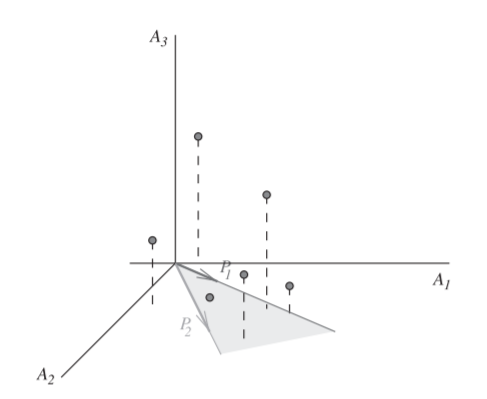
\includegraphics[width=0.4\textwidth]{img/espacio02.png}
\caption{Representación de tres n-alcanos ($A_1$,$A_2$,$A_3$), dos especies de plantas (vectores $P_1$ y $P_2$), y seis muestras de heces (puntos de la figura), dando lugar a un cono bidimensional generado por los dos vectores de plantas.}
\label{fig:espacio02}
\end{figure}

Por tanto, siempre que el número de especies supere al número de n-alcanos se suele enfocar el problema agrupando las especies en categorías. Sin embargo, no existe un claro criterio satisfactorio para decidir cómo agrupar las especies (cómo definir una partición $d$ al conjunto de vectores $P_1, P_2,...,P_p$) ni cómo ponderarlas dentro de cada grupo.

Para resolver este problema se sugiere un enfoque alternativo que usa números arbitrarios de especies de plantas y n-alcanos.

\begin{figure}[h!] 
\centering
    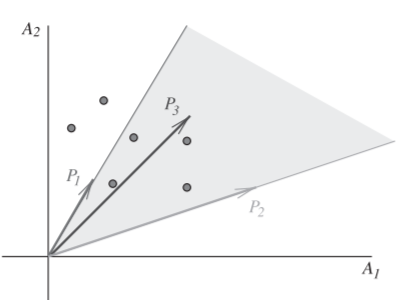
\includegraphics[width=0.4\textwidth]{img/espacio03.png}
\caption{Representación de dos n-alcanos ($A_1$,$A_2$), tres especies de plantas (vectores $P_1$, $P_2$ y $P_3$), y seis muestras de heces (puntos de la figura). El área sombreada es el cono bidimensional generado por los vectores $P_1$, $P_2$ y $P_2$..}
\label{fig:espacio03}
\end{figure}

Partiendo de $P_1, P_2,...,P_p$ vectores de $d$ componentes que representan $p$ plantas, donde $d$ es el número de n-alcanos usados, y $C$ el cono generado por los vectores, denotamos $F_i = 1,2,...,q$ la proyección en $C$ del punto en $d$, y definimos $\phi$ como el conjunto de muestras fecales \textit{``correctas''}.

Definimos una dieta factible, aquella solución no negativa del sistema lineal $Ax=F$, para cualquier punto de $F$ en $\phi$, donde $A$ es $d \times p$ matriz con columnas $P_1, P_2,...,P_p$. Hay muchas dietas factibles. No obstante, el conjunto de dietas está acotado por \textbf{límites superiores e inferiores} para cada uno de los coeficientes, la programación lineal es una herramienta adecuada para abordar algunas de las siguientes cuestiones sobre la dieta:

\begin{itemize}
    \item ¿Cuáles son las proporciones máximas y mínimas de cada especie en la dieta?
    \item ¿Cuáles son las proporciones máximas y mínimas de cada grupo en la dieta?
    \item ¿Cuál es la proporción mínima de una planta, en concreto  en aquellas dietas que cumplen un requisito (por ejemplo, los niveles de ingesta de nitrógeno o tanino contenido)?
\end{itemize}




\capitulo{4}{Técnicas y herramientas}

Esta parte de la memoria tiene como objetivo presentar las técnicas metodológicas, bibliotecas, lenguajes y las herramientas de desarrollo que se han utilizado para llevar a cabo el proyecto. Se comentarán los aspectos más destacados de cada opción y se han añadido referencias bibliográficas que incluyen más información.

\section{Herramientas de metodología ágil}
\textbf{Git}

Git es un software de control de versiones (free and open source) diseñado por Linux Torvalds, centrado en la eficiencia, confiabilidad y compatibilidad del mantenimiento de versiones de aplicaciones con una gran cantidad de archivos de código fuente. 

La característica diferencial con el resto de SCM\footnote{\textbf{Gestión de configuración de Software} (Software Configuration Management, SCM) es una especialización de la gestión de la configuración de todas las actividades en el sector de desarrollo de software. SCM trata y controla: La elaboración de código fuente por varios desarrolladores simultáneamente} es su modelo de ramificación, permitiendo trabajar en ramas locales, para después poder realizar operaciones de fusión y eliminación del código con facilidad.

%\imagen{git_branches}{Ramificación git} 

Para más información: \url{https://git-scm.com/}

\textbf{GitHub} 

Github es una plataforma destinada a alojar proyectos para el control de versiones Git y desarrollo colaborativo software. 

Hemos utilizado GitHub debido a su facilidad de cara a trabajar con la metodología SCRUM, permitiéndonos dividir el proceso de desarrollo en períodos de trabajo o "sprints", y realizar análisis posteriores que nos mostrarán posibles errores de planificación y aciertos en cuanto al desarrollo del proyecto. Otro factor es su facilidad de interacción con otras herramientas.

Repositorio del proyecto en GitHub: \url{https://github.com/humbertoms99/DIET_COMPOSITION}

\textbf{ZenHub}

Para realizar el seguimiento de los desarrollo del proyecto se ha utilizado ZenHub, que es un extensión de Chrome que se integra de forma nativa en la interfaz de usuario de GitHub, y nos  ofrece un seguimiento de los requerimientos de nuestros repositorios. Nos permite realizar planificaciones junto con un seguimiento y posterior análisis. También incluye filtrado por etiquetas, agrupación de problemas, visualizar posibles bloqueadores, entre otras opciones. 

Conviene destacar la facilidad con se crean los gráficos de ejecución, seguimiento de la velocidad e informes de versión. Estos se  analizarán en los anexos de este proyecto.

Para más información: \url{https://www.zenhub.com/}

\section{Lenguajes de programación}


\textbf{HTML}

Es un lenguaje de marcado de hipertexto dedicado a la elaboración de código utilizado para estructurar y desplegar  páginas web.
HTML se escribe en forma de etiquetas rodeadas por corchetes angulares (<,>,/). Hemos utilizado este lenguaje en el proyecto de front-end  para realizar las vistas de nuestra web.

\textbf{Typescript}

Es un lenguaje fuertemente tipado basado en JavaScript. Se diferencia respecto a JavaScript en que añade tipos estáticos y objetos basados en clases.

\textbf{PHP}

Es un lenguaje de código abierto adecuado para desarrollo web y que puede ser incrustado en HTML. Lo que distingue a PHP es que el código se ejecuta en el servidor, al contrario que en lenguajes como Javascript, que se ejecutan del lado del cliente.

Para más información: \url{https://www.php.net/manual/es/}

\textbf{CSS}

Es un lenguaje de diseño gráfico o lenguaje de estilos para definir la presentación de un documento estructurado escrito en lenguajes de marcados (HTML o XML). Es uno de los lenguajes base para Webs; con él podemos alterar la fuente, color, tamaño y espaciado del contenido.

\textbf{JSON}

Es un formato de texto utilizado en el intercambio de datos. Se trata de un subconjunto de notación de objetos de JavaScript.
Este tipo de formato es el esperado al hacer peticiones a la API desde nuestro front en Angular, permitiendo enviar estructuras de datos que pueden ser leídas con facilidad.

\section{Patrones de diseño}

\textbf{MVC}

MVC (Modelo-Vista-Controlador) es un patrón de diseño de software utilizado para implementar interfaces de usuario, datos y lógica de control. Su característica  principal es la separación de código en tres partes:
\begin{enumerate}
	\item Modelo: contiene la representación de los datos y lógica de negocio.
	\item Vista:  diseño de la interfaz gráfica de usuario; contiene la información que se envía al cliente.
	\item Controlador: Actúa como intermediario entre Modelo y Vista, gestionando y transformando los datos.
\end{enumerate}

En el caso particular del desarrollo web, el modelo suele corresponder al propio \emph{"model"} de una tabla de base de datos, el  código suele estar escrito en Javascript, y la vista  en HTML / CSS.

\section{Frameworks y servicios}

\textbf{Visual Studio Code}

Es un editor de código fuente  que se ejecuta en Windows, macOS y Linux. Incluye soporte  para la depuración control integrado de Git. Algunas características que ofrece el framework:

1. IntelliSense, que es un conjunto de funcionalidades de edición de código como sugerencias  de métodos y propiedades de objeto, información de parámetros y sus tipos.

2. Depuración directa desde el editor. Visual Studio Code ofrece depuración de código con puntos de  interrupción, pilas de llamadas y una consola interactiva.

3. Comandos git incorporados, permitiendo realizar revisiones en el propio framework, pudiendo descartar cualquier servicio SCM alojado.
% [TODO NOTA A PIE Supply Chain Management]

4.  Una gran cantidad de extensiones que facilitan el rápido desarrollo y visualización del código.

5. Implementación y posibilidad de alojar sitos en React, Angular, Vue, Node, Python entre otros, además de almacenar y consultar datos relacionados.

Para más información: \url{https://code.visualstudio.com}

\textbf{Postman}

Postman es una plataforma de API que permite a los  desarrolladores testear sus APIs. Nos ofrece la posibilidad de simular peticiones HTTP request a través de una interfaz gráfica adaptada al usuario, por la cual podremos observar el estado de la respuesta y de los datos que se obtienen, posibles mensajes de validaciones. 

\begin{figure}[h!] 
\centering
    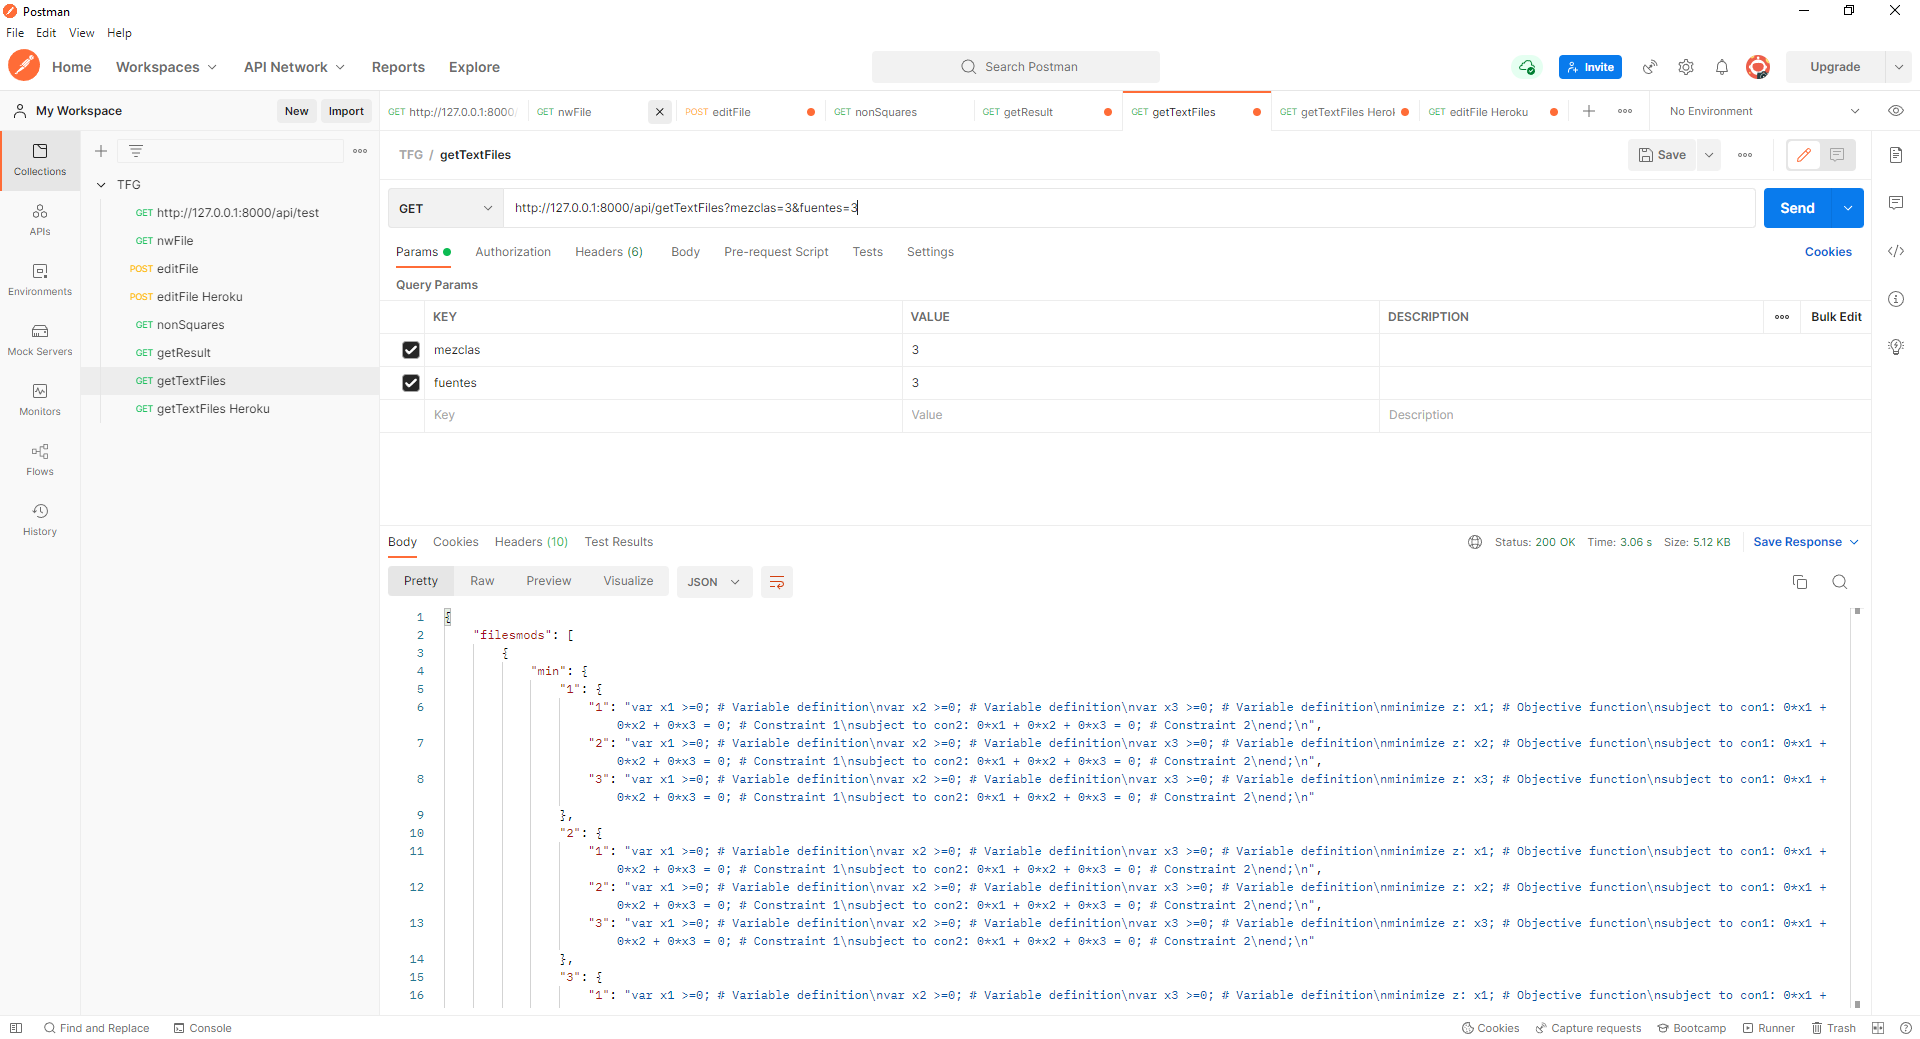
\includegraphics[width=1\textwidth]{img/postmanRequest.PNG}
\caption{Petición Postman}
\label{fig:request_postman}
\end{figure}

En la Figura \ref{fig:request_postman} se puede observar la interfaz de Postman, en la cual podemos organizar nuestras peticiones en Colecciones; a la derecha encontramos la url a la que se realiza la petición y el tipo operación. En la parte central nos permite introducir parámetros (hemos comprobado que ofrece la opción de introducir textos JSON  como parámetros). También nos ofrece la opción de configurar los headers y pasar un token en caso de nuestra API trabaje con un login previo.

Al lanzar la petición, retorna la repuesta en la parte inferior de la interfaz. En la esquina superior derecha se encuentra el status , es decir, si se ha realizado correctamente o si ha  llegado a un estado fallido (status 200: OK, status 4XX: Error en la petición al cliente, status 5XX: Error en el servidor).

El \textit{body} de la respuesta puede ser consultado en los siguientes formatos de texto: JSON, XML, HTML, Text o Auto, según nuestra elección.

Para más información: \url{https://www.postman.com/}

\textbf{Debian}

Debian es un sistema operativo libre desarrollado por la comunidad a través de la colaboración voluntaria. Hemos utilizado este subsistema a modo de terminal Linux para poder instalar la librería GLPK. Hemos seleccionado este sistema debido a compatibilidad  y facilidad de instalación desde Windows, que es el sistema operativo donde se han realizado los desarrollos del proyecto.

Para más información: \url{https://rincondelatecnologia.com/subsistema-linux-en-windows-10-que-es-para-que-sirve-y-como-instalarlo/}

%TODO: alternativas ubuntu otras terminales linux

\textbf{Angular}

Angular es un framework de JavaScript de código abierto, mantenido por Google, que se utiliza para  crear aplicaciones web \textit{Single Page Application}. Angular trabaja con el patrón de diseño MVC al ofrecer una separación clara entre las vistas y las funciones que realizan las operaciones con los datos, separando el lado del cliente del lado servidor. 

Angular está formado por un conjunto de herramientas para la interfaz de nuestra aplicación web; destaca su capacidad de adaptación permitiendo modificar sus características según el flujo de trabajo lo requiera, además de tener facilidad para incorporar otras librerías

Para más información: \url{https://www.udemy.com/course/angular-fernando-herrera}

\textbf{Angular Translate}

Angular translate es un modulo de Angular, que nos ha permitido internacionalizar la web a través de traducciones dinámicas. Su funcionamiento es por medio del pipe \textit{translate}, que busca el texto introducido en la carpeta \textit{i18n/**.json} y muestra su traducción correspondiente. En la figura \ref{fig:angular_translate} se realiza una traducción de la línea $26$ al inglés, añadiendo el pipe \textbf{translate} e incorporando el texto en el archivo de traducciones \textit{en.json} (Línea 3).

\begin{figure}[h!] 
\centering
    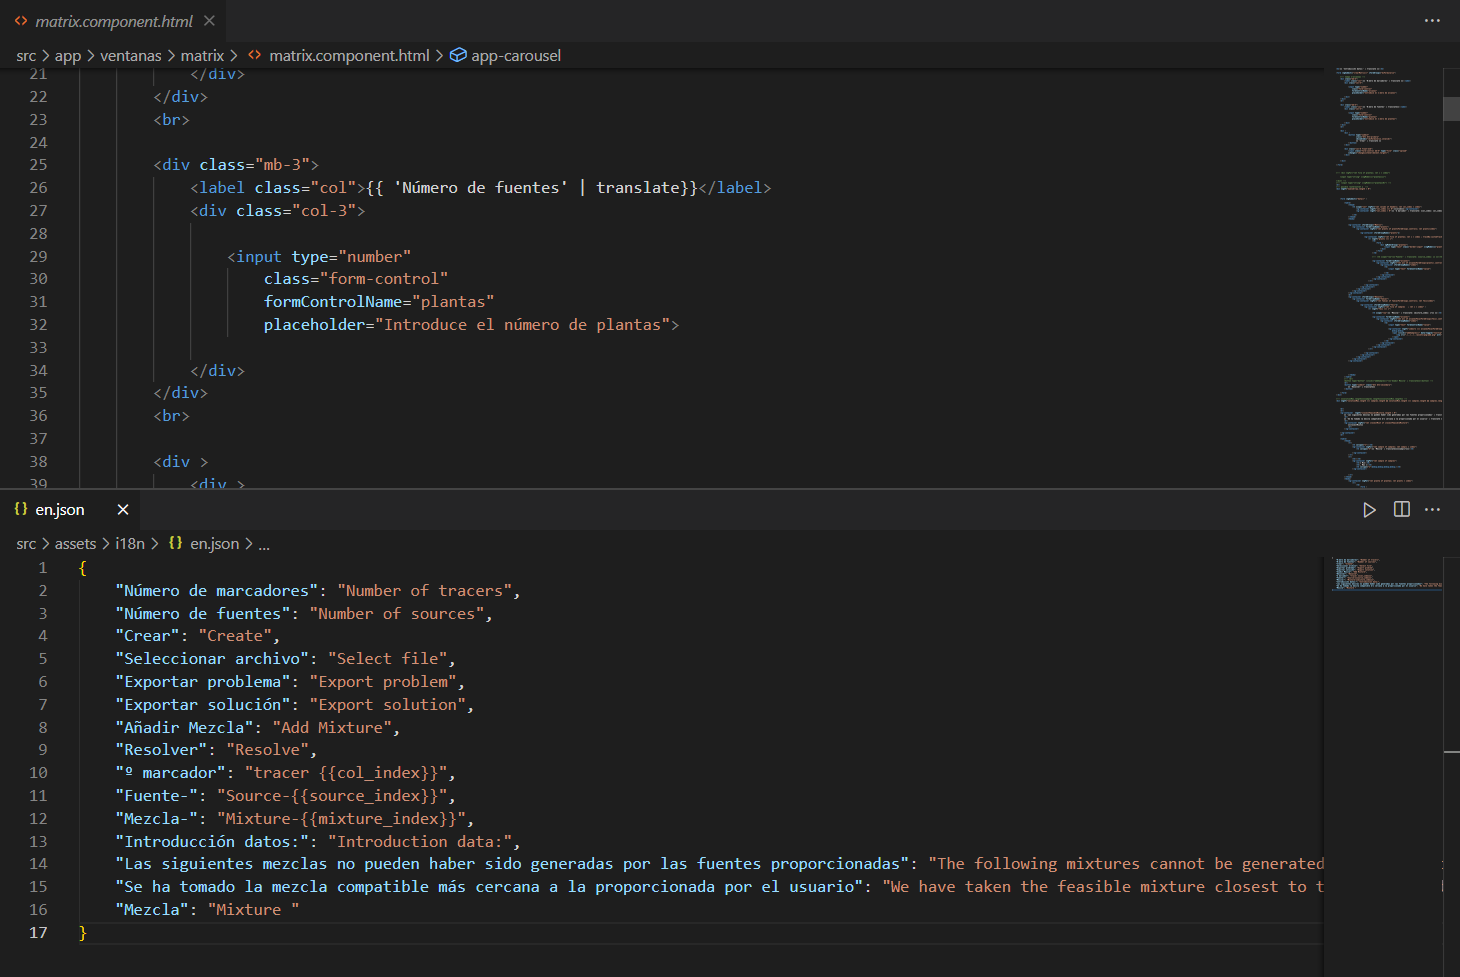
\includegraphics[width=0.8\textwidth]{img/translate.PNG}
\caption{Ejemplo Angular Translate}
\label{fig:angular_translate}
\end{figure}

\textbf{Angular Material}

Angular Material es un modulo de Angular, este modulo ofrece una biblioteca de componentes de interfaz de usuario (UI), los desarrolladores añaden estos componentes al modulo de Angular Material que a su vez es utilizado por el proyecto. Estos componentes nos  ofrecen interfaces de usuarios elegantes  y reutilizables, algunos componentes pueden ser botones, select, checkbox, table, Dialog, entre otros muchos.

Para trabajar con los componentes ofrecidos se ha seguido su documentación: \url{https://material.angular.io/components/categories}

\textbf{Bootstrap}

Bootstrap es una biblioteca multiplataforma o conjunto de herramientas de código abierto  para diseño de sitios y aplicaciones web. Incluye diseños plantilla para componentes habituales de las web, al igual que Angular Material. Una de sus características es su diseño adaptativo (\textit{"Responsive Design"}), que consiste en adaptar el diseño  de la aplicación a los distintos tamaños  de pantallas, permitiendo así acondicionar nuestras interfaces a los posibles cambios en el tamaño de pantalla.

Además ofrece la posibilidad de incluir esta librería por via CDN, que consiste en añadir un link en el archivo \textit{index.html} y carga automáticamente los estilos de bootstrap en la aplicación.


\textbf{Node.js}

Node.js es un entorno de ejecución para JavaScript construido con V8, basado en el motor de JavaScript de Chrome, con E/S de datos en una arquitectura orientada a eventos, y que utiliza un único hilo de ejecución asíncrono.

Para más información \url{https://nodejs.org/es/}

\textbf{npm}

Npm es un sistema de gestión de paquetes por defecto para Node.js. Coloca los módulos en su lugar para que Node pueda encontrarlos y gestionar los conflictos eficientemente.

Npm es muy configurable algunas de sus funcionalidades más comunes son la publicación, búsqueda, instalación y desarrollo de programas  node.

Con vista a la instalación de librerias, npm tiene dos modos: 
\begin{itemize}
	\item modo  global: npm instala los paquetes en \textit{prefix/lib/node\_modules} y los bins en \textit{prefix/bin}.
	\item modo local: npm instala los paquetes en el directorio del proyecto actual. Los paquetes en la ruta \textit{./node\_modules}, y los bins en ./bin.
\end{itemize}

\textbf{Heroku}

Heroku es una plataforma como  (PaaS) de computación en la Nube que soporta distintos lenguajes de programación. Heroku es propiedad de Salesforce.com. y ofrece servicios gratuitos para el despliegue proyectos.

Se ha utilizado para realizar el despliegue del back-end escrito en php en un servidor. 

\textbf{Netlify}

Netlify es una empresa  informática en la nube con sede en San Francisco que ofrece alojamiento a servicios para aplicaciones web y sitios estáticos.

En nuestro caso hemos hecho uso del paquete Starter gratuito para uso individual, y hemos desplegado el front-end en Angular, que llama a la API. .

\section{Librerias}

\textbf{glpk-5.0}

GLPK (GNU Linear Programming Kit) es un paquete destinado a resolver problemas de programación lineal, programación de enteros mixtos y otros problemas relacionados. Es un conjunto de rutinas  escritas en ANSI C y organizadas en forma de biblioteca invocable.

Se ha usado esta  librería en el back-end para resolver problemas de programación  linear mediante comandos que se ejecutan en una terminal Linux y tienen como resultado la generación de archivos .mod. Posteriormente veremos el análisis de estos archivos y datos requeridos para realizar el cálculo.

Para más información: \url{https://www.gnu.org/software/glpk/}

\textbf{libtsnnls-2.3.4}

Libtsnnls es un paquete de node que resuelve el problema de Fast Combinatorial Non-negative Least Squares. Se ha realizado la instalación con su comando  de instalación npm \textit{"npm i ml-fcnnls"} en el proyecto front y se ha usado para calcular las proyecciones de los puntos en el cono formado por las fuentes.

Para más información: \url{https://www.npmjs.com/package/ml-fcnnls/v/1.0.0}


\section{Otras Herramientas}

\textbf{Latex: TexStudio}

TexStudio es un editor de Latex de código abierto y Multiplataforma con una interfaz similar a Texmaker, que proporciona un soporte moderno de escritura, ofrece corrección ortográfica, plegado de código y resaltado de sintaxis. Ha aportado una revisión de la sintaxis de los documentos escritos en Latex.

Para más información: \url{https://www.texstudio.org/}


\textbf{Mendeley}

Mendeley es un gestor de referencias que se utiliza para administrar y compartir trabajos de investigación y la generación de bibliografías para artículos académicos. Se ha utilizado su aplicación de escritorio  \textit{Mendeley Reference Manager}.

Para más información: \url{https://www.mendeley.com/?interaction_required=true}


\textbf{Draw.io}

Draw.io es un software de dibujo gráfico  multiplataforma  gratuito y de código abierto desarrollado en HTML5 y JavaScript. Su interfaz permite crear diagramas de flujo, wireframes, diagramas UML, organigramas y diagramas de red. Se ha trabajo desde su versión online, y se ha elegido como  herramienta debido a su facilidad de uso y la cantidad de opciones de diseño que ofrece.

\textbf{Overleaf}

Overleaf es un  editor de textos Latex online que se utiliza para publicar documentos científicos, Se ha usado para realizar la documentación de este proyecto. Algunas ventajas respecto a otros editores es su  guardado en nube automático y permite auto compilación del código lo que nos proporciona una mayor agilidad a la hora de documentar.

Para más información: \url{https://es.overleaf.com/learn}

\section{Uso de herramientas}

En la tabla \ref{fig:herramientasportipodeuso} podemos ver un resumen visual de las herramientas que hemos usado en cada apartado del proyecto.

\begin{itemize}
	\item \textbf{Planificación y metodología}.
	\item \textbf{APP Angular}: aplicación de tipo single-page application, que se divide en componentes con archivos TS / HTML / CSS / TEST por componente.
	\item \textbf{API}: Proyecto que contiene estructura modelo-vista-controlador (en este caso solo se ha  trabajado con controladores, al haber considerado que no era necesario guardar datos en bases de datos y por tanto no ser necesario el modelo).
	\item \textbf{Memoria}: documentos memoria y anexos escritos en \LaTeX{}.
\end{itemize}

\begin{table}[h]
    \rowcolors{1}{}{lightgray}
    \centering
    \begin{tabular}{l c c c c}
        \textbf{Herramientas} & Planificación & App Angular & API & Memoria \\ 
        \hline
        Git & X & & &\\
        GitHub & X & & & \\
        ZenHub & X & & &\\
        HTML & & X & &\\
        Typescript & & X & &\\
        PHP & & & X &\\
        CSS & & X & &\\
        JSON & & X & X &\\
        Visual Studio Code & & X & X & X\\
        Postman & & X & X &\\
        Debian & &  & X &\\
        Angular & & X & &\\
        Angular Translate & & X & &\\
        Angular Material & & X & &\\
        Bootstrap & & X & &\\
        Node.js & & X & X &\\
        npm & & X & X & \\
        Heroku & & & X &\\
        Netlify & & X & &\\
        GLPK & & X & X & \\
        libtsnnls & & X & &\\
        \TeX{}Studio & & & & X\\
        Mendeley & & & & X\\
        Draw.io & & & & X\\
        Overleaf & & & & X\\
    \end{tabular}
    \caption{Herramientas y tecnologías utilizadas en cada parte del proyecto}
    \label{fig:herramientasportipodeuso}
\end{table}














\capitulo{5}{Aspectos relevantes del desarrollo del proyecto}

Este apartado pretende recoger los aspectos más interesantes del desarrollo del proyecto, la exposición del ciclo de vida, y detalles de mayor relevancia en las fases de análisis, diseño e implementación.

\section{Inicio del proyecto}


En una primera reunión se realizó una primera  discusión sobre el artículo \cite{problemn-alkanes2007}, para entender los objetivos reales del proyecto. 

A partir de este momento se buscaron opciones para llevar a cabo el desarrollo de una web que realizara operaciones de programación lineal para calcular las composiciones de la dieta de grupos de animales (más adelante se entendió que realmente  esta implementación  permitía resolver otros muchos problemas dentro del marco de los \emph{Mixing Models}). Las dos grandes alternativas a la hora de desarrollar la web fueron React vs Angular.

\section{Selección React vs Angular}

Con el objetivo de ordenar y aclarar diferencias entre React y Angular se ha realizado la tabla \ref{tab:reactvsangular}.

\begin{table}[h]
    \centering
    \begin{tabular}{| m{2.5cm} | m{5cm} | m{5cm} |}
    \hline
        Característica & React & Angular \\ \hline
        ¿Que es? & Javascript framework & Javascript biblioteca para el desarrollo de interfaces gráficas \\ \hline
        Tipo de Webs & Web y móvil, Single- y Multiple-page applications & Web y móvil, Single- y Multiple-page  applications\\ \hline
        Aprendizaje & Largo y difícil & Rápido y simple si se conoce Javascript previamente\\ \hline
        Comunidad & Grande & Grande\\ \hline
        Rendimiento & Optimizado con detección de cambios & Optimizado con virtual DOM\\ \hline
        Lenguajes & JavaScript, TypepScript & JS ES6+, JSX script\\ \hline
        Estructura de la APP & Fijo y complejo, componentes basados en MVC & Flexible, componentes  basados en vistas\\ \hline
        Directivas & Incomprensibles sin conocimiento previo en Angular & Fáciles de entender con conocimiento en Javascript\\ \hline
        Vinculación de datos & Bidireccional, datos mutables & Unidireccional, datos  inmutables\\ \hline
        Herramientas & Aptana, Sublime Text, Visual Studio, Angular CLI, Angular Universal, Jasmine,  Protractor, Karma & Sublime Text, Visual Studio, Atom, Create React App (CLI), Next.js framework, Enzyme, Hest, React-unit\\ \hline
        Añadir librerias en Javascript en el código & Posible & No posible\\ \hline
    \end{tabular}
    \caption{Comparativa entre React y Angular. Fuente: Elaboración propia}
    \label{tab:reactvsangular}
\end{table}

\newpage

Inicialmente, el lenguaje más atractivo era React por su facilidad de aprendizaje y uso.
Un punto que nos preocupaba tanto a mí como a los tutores en cuanto al diseño de la web, era que fuera Single-page-application, opción que permiten los dos lenguajes. 
Por parte de los lenguajes de programación, se partía de cero en los dos casos, al yo no tener conocimientos previos en Javascript ni en Typescript.
En cuanto a la estructura de la APP, el MVC ha sido estudiado en algunas asignaturas durante la carrera, habiéndole dado más importancia que modelos basados únicamente en vistas.
Respecto a las herramientas, se conocían con anterioridad Sublime Text y Visual Studio, que son comunes en los dos lenguajes y no tienen una gran importancia en cuanto al uso exclusivo de un lenguaje, al ser los dos editores de textos.

En este caso, hubo un punto más a tener en cuenta, y es que durante este año he estado realizando prácticas en una empresa, y el lenguaje con el que se ha trabajado ha sido Angular, de modo que para reducir tiempos de formación y trabajar en un lenguaje un poco más conocido se decidió seleccionar Angular como el lenguaje principal para el desarrollo del proyecto al no tener previamente una mayor diferenciación a parte de su simplicidad de aprendizaje por parte de React.

\section{Metodología}

La metodología utilizada ha sido SCRUM, metodología aprendida en la asignatura de \emph{Gestión de Proyectos}. SCRUM es un marco de trabajo para desarrollo ágil, el cual son un conjunto de buenas prácticas para trabajar de forma colaborativa y obtener el mejor resultado  posible.

Algunas de las medidas características de la metodología que se han aplicado en el proceso de desarrollo son:

\begin{itemize}
	\item La  planificación del desarrollo se ha realizado en periodos de una misma duración con objetivos claros, llamados \emph{"sprints"}. Estos se encuentran en el repositorio de GitHub \url{https://github.com/humbertoms99/DIET_COMPOSITION}.
	\item El desarrollo  de la aplicación ha sido incremental.
	\item Se han mantenido reuniones al final de cada sprint para hablar de las implementaciones y próximos desarrollos. 
	\item Se ha estimado el valor de los objetivos de los \emph{sprints}  mediante Story points. 
	\item Se han añadido, movido y completado tareas mediante la herramienta Zenhub.
	\item Se ha establecido un tiempo de 2 semanas por cada sprint.
\end{itemize}

\section{Desarrollo del proyecto}

Durante las primeras semanas se realizó un curso de \LaTeX{} \cite{curso:latex}, con el objetivo de documentar las elecciones entre herramientas. 

Posteriormente  se pasó a documentar el problema planteado en el articulo \cite{problemn-alkanes2007} sobre el problema de n-alcanos, siendo el objetivo inicial del proyecto.

Uno de los objetivos más importantes para el funcionamiento del proyecto fue el uso de una biblioteca que resolviera problemas de programación lineal, como \cite{glpk:package}. El proceso de instalación y configuración de esta biblioteca conllevó algunos problemas: el primer problema fue la necesidad de ejecutar algunos comandos de la instalación desde una terminal Linux. Al estar trabajando en un entorno Windows se decidió continuar en el sistema operativo,  por lo que se optó  por usar una herramienta que actuara como subsistema  Linux en Windows 10, en este caso Debian \cite{debian}, al ser este un software gratuito y con distribución libre.

Otro problema que surgió durante la configuración de la librería fue el requerimiento de un compilador en C, ya que la librería está escrita en ANSI C, lo cual se resolvió con siguiendo los pasos de una respuesta encontrada en StackOverFlow \cite{stack:Compiler}. Otro punto a destacar sobre el uso de esta librería, es que requiere  que el servidor se este ejecutando en una terminal Linux, por lo que se configuró Visual Studio Code para escribir comandos en una terminal Linux.

Una vez entendidos los objetivos del problema a resolver y disponer de una librería que resolviera estos requerimientos, comenzó la fase  de implementación, dividiendo esta parte del desarrollo en periodos muchos más marcados con requisitos claros y trabajando simultáneamente en el proyecto front-end en Angular y el back-end en un proyecto laravel. A continuación analizaremos algunos de los puntos que consideramos claves de implementación.

\subsection{Formularios}

Angular ofrece dos técnicas para crear formularios: formularios basados en plantillas (Template Forms) y formularios reactivos (Reactive Forms). 

Se optó por realizar los formularios  reactivos, al ser más sencillos, ya que las validaciones se trabajan desde la clase componente siendo  una lógica más limpia, al pasar las validaciones al componente. Al contrario que los formularios por plantilla, es más fácil definir formularios dinámicos (punto importante al trabajar con una matriz que va cambiar de tamaño).

La diferencia principal es que los \emph{Reactive Forms} definen el formulario en la clase del componente y trabajan  en la vista con las directivas \emph{formGroup} o \emph{formControlName},  al contrario que los \emph{Template Forms}, donde las reglas y estructura del  formulario se hacen en la vista utilizando directivas como \emph{ngForm} y \emph{ngModel}

Para mantener la idea de separación entre vista y lógica, se decidió utilizar los \emph{Reactive Forms}, que además son más fáciles de usar y permiten más adaptaciones por parte de las validaciones.

\begin{figure}[h!] 
\centering
    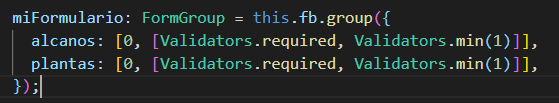
\includegraphics[width=0.8\textwidth]{img/formIndexMatrix.PNG}
\caption{Fórmulario index Matrices}
\label{fig:formIndexMatrix}
\end{figure}

En la figura \ref{fig:formIndexMatrix} se puede ver el código de clase del componente que contendrá los índices de la matriz de datos a solicitar posteriormente. Estos campos son siempre requeridos y deben tener un valor superior a "1"; por el contrario, el botón de crear matrices permanecerá deshabilitado.

\begin{figure}[h!] 
\centering
    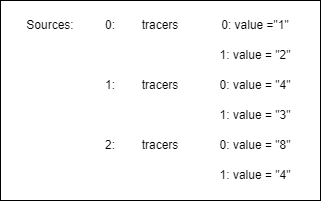
\includegraphics[width=0.8\textwidth]{img/formSources.png}
\caption{Estructura de datos del formulario que contiene los valores de las fuentes}
\label{fig:formSources}
\end{figure}

En la Figura \ref{fig:formSources} podemos observar la estructura del segundo formulario que contendrá los datos de la matriz de datos con los valores de los marcadores para cada fuente. La estructura de este formulario es un "\textit{array de Sources}"  que tendrá tantos elementos como fuentes se especifiquen en los \textit{index} del anterior formulario. Cada elemento está formado por un único \textit{formArray} de marcadores (tantos como se especificaron en el primer formulario). En este último array se encuentran los correspondientes valores de cada marcador para la fuente.

\begin{figure}[h!] 
\centering
    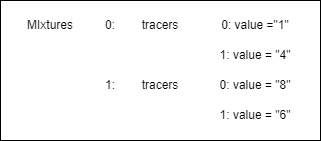
\includegraphics[width=0.8\textwidth]{img/formMixtures.png}
\caption{Estructura de datos del formulario que contiene los valores de las mezclas}
\label{fig:formMixtures}
\end{figure}

En la Figura \ref{fig:formMixtures}  observamos la estructura de datos del tercer formulario que contiene los datos de las mezclas sobre las cuales queremos calcular el problema. Estos datos son rellenados mediante la interfaz al usar el botón de añadir mezcla. La estructura del formulario es un "\textit{array de Mixtures}"  que tendrá tantos elementos como mezclas se crean en la interfaz. Cada elemento esta formado por un único \textit{formArray} de marcadores (tantos como se especificaron en el primer formulario). En este último array se encuentran los correspondientes valores de cada marcador para la fuente.

Por último, se implementó un cuarto formulario que permite  el cambio de nombre de las fuentes, con el objetivo de hacer más visible las posibilidades de resolver el problema de los \textit{Mixing Models}.

\subsection{Estructura documentos csv}

En esta sección visualizaremos los archivos .csv exportados por la aplicación web y  explicaremos su estructura.

\subsubsection{Export Input Data}

En la Figura \ref{fig:inputData} podemos ver una vista de los datos que corresponden al archivo \textit{InputData.csv}; este archivo será el esperado en la opción de importar datos.

Las dos primeras filas marcan el número de marcadores y fuentes  respectivamente. A continuación, siempre se dejará una línea vacía que marca que las siguientes líneas son los valores para cada fuente; el número de filas de fuentes corresponderá al número de fuentes fijado en la segunda fila. Para diferenciar las filas referentes a los valores de las mezclas  se deja otra fila vacía. Es obligatorio dejar estas filas vacías para que la entrada de los datos sea correcta.

\begin{figure}[h!] 
\centering
    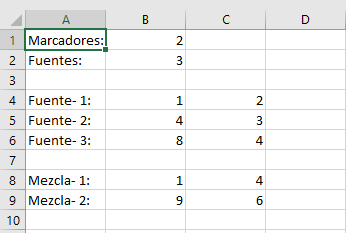
\includegraphics[width=0.8\textwidth]{img/inputData.PNG}
\caption{Vista csv InputData}
\label{fig:inputData}
\end{figure}

\subsubsection{Export Solution}

En la figura \ref{fig:solution} podemos ver la vista de  la solución del problema. Se ha intentado que mantuviera una disposición similar a la de la aplicación web. En una primera parte tenemos los datos del problema tal cual se encuentran en el archivo \textit{InputData.csv}. Posteriormente se añade una línea con la proyección de la muestra usada para realizar el calculo.

Por último, podemos  apreciar una estructura de tabla en la cual podemos ver las estimaciones máximas y mínimas de las mezclas sobre las fuentes.

\begin{figure}[h!] 
\centering
    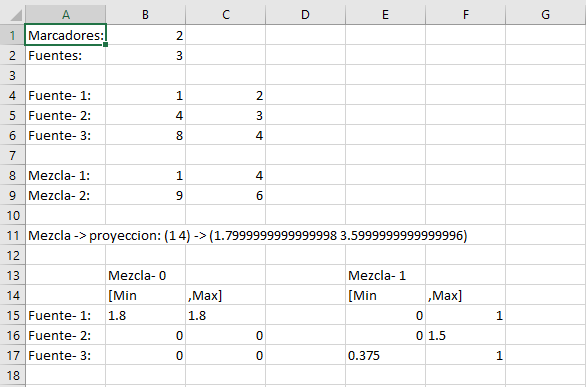
\includegraphics[width=0.8\textwidth]{img/solution.PNG}
\caption{Vista csv Solution}
\label{fig:solution}
\end{figure}

\subsubsection{Export Paso Intermedio }

En el caso de los dos tipos de exports vistos previamente, la descarga era trivial  ya que se mostraban sus pertinentes botones de exports una vez realizado el cálculo. En el caso de que queramos ver los cálculos intermedios realizados para cada valor, sera necesario dar click sobre el propio valor de estimación tanto para máximos, que descargará un archivo con nombre \textit{M1\_max1.csv}, como para mínimos, donde el fichero se llamará \textit{M1\_min1.csv}. El nombre es una simplificación de "Mixture 1 - Maximize Source 1".

El contenido de la Figura \ref{fig:pasoIntermedio} corresponde con los archivos \textit{.mod} usados desde la API para resolver el problema de maximización de un objetivo sobre un conjunto de reglas y ecuaciones. La segunda columna  marca el tipo de línea que es, teniendo líneas para la definición de las variables: una  única línea que señaliza el tipo de operación (maximización o minimización) y la función objetivo, y unas últimas líneas que contendrán las ecuaciones con los índices de los marcadores tanto para fuentes como para las mezclas

\begin{figure}[h!] 
\centering
    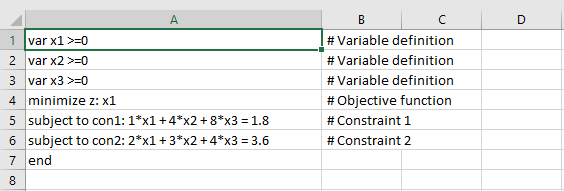
\includegraphics[width=0.8\textwidth]{img/pasoIntermedio.PNG}
\caption{Vista csv paso intermedio}
\label{fig:pasoIntermedio}
\end{figure}

\newpage
\section{Ciclo de la aplicación}

En este apartado vamos a comentar los pasos que realiza la aplicación y nos detendremos en los que consideremos más importantes

Al entrar a la web en la parte superior veremos un \textit{"Top Navigation Bar"} \cite{Navigation:Bar}, donde la primera ventana ha sido dedicada a la resolución del problema, una segunda con un vídeo guía de uso de la aplicación, el icono con enlace directo al GitHub y finalmente un apartado de las personas participantes en el desarrollo del proyecto.
Justo debajo encontraremos el primer formulario con dos inputs para introducir los índices de la matriz de fuentes. junto con dos botones:  botón \textit{``Crear''} y  \textit{"Seleccionar archivo"}. Este segundo lanza un evento y permite leer archivos con el formato esperado.

Estos dos botones marcan las dos alternativas del flujo en la Figura \ref{fig:cicloDeVida}. En el caso de la rama izquierda del flujo  (\textit{``Introducción manual de los datos''}) es necesario rellenar el primer formulario con los índices, un segundo con los valores de las fuentes y dar valores para las mezclas (pudiendo añadir más mezclas con su botón correspondiente).

Estos dos flujos se unen al dar al botón \textit{``Resolver''}. Al hacer click se calcularán las proyecciones de las mezclas, y en caso de ser diferentes a las mezclas originales se mostrará un mensaje en pantalla con los valores sobre los que se han realizado los cálculos. 



\begin{figure}[h!] 
\centering
    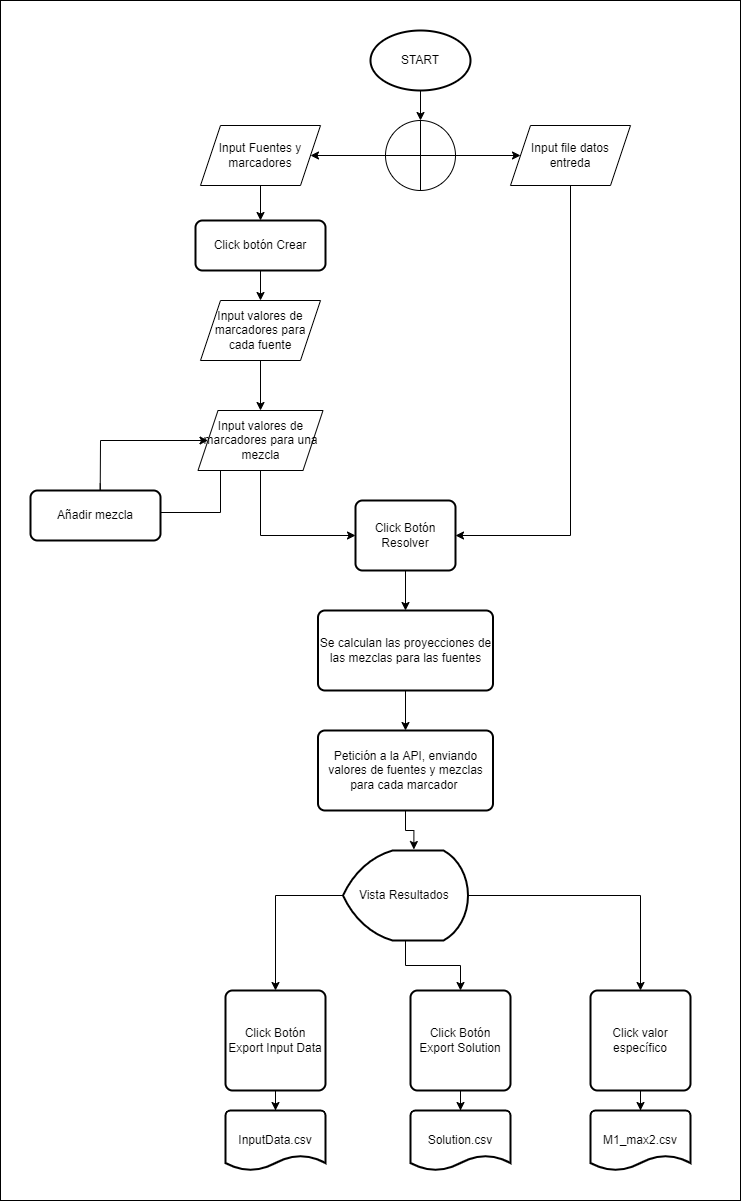
\includegraphics[width=0.8\textwidth]{img/cicloDeVida.png}
\caption{Ciclo de vida }
\label{fig:cicloDeVida}
\end{figure}

Una vez se han calculado las proyecciones de las mezclas, se ejecuta una petición por cada mezcla con los arrays de fuentes y valores para la mezcla al API. Esta petición genera un archivo tipo \textit{"file\_max1\_1.mod"} en la ruta \textbf{storage/app} del  proyecto en laravel por cada marcador que tiene cada mezcla. Su contenido es equivalente al mostrado en la figura \ref{fig:pasoIntermedio}. Para resolver el problema de maximización o minimización, hacemos uso de la librería \cite{glpk:package} con el comando \textit{"glpsol -m ../storage/app/file\_max1\_1.mod -o files\_sol/file\_max1\_1.sol"} que nos genera un archivo tipo \textit{".sol"}. Este comando requiere  ser ejecutado desde una terminal Linux (En el entorno local se uso debian wsl \cite{debian}); este comando genera un archivo tipo \textit{".sol"} en la ruta \textit{public/files\_sol/}.

\begin{figure}[h!] 
\centering
    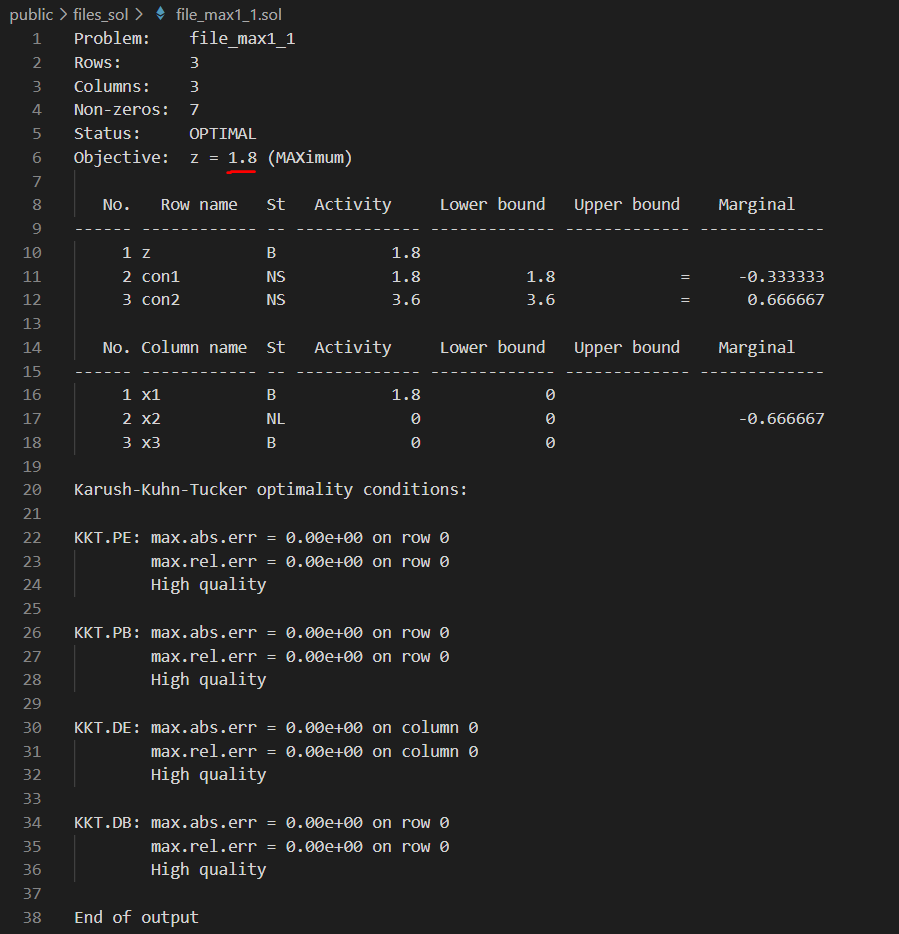
\includegraphics[width=0.8\textwidth]{img/fileSol.PNG}
\caption{Archivo file\_max1\_1.sol }
\label{fig:fileSol}
\end{figure}

Dicho archivo, denominado \textit{file\_max1\_1.sol}, devuelve el valor objetivo calculado en la línea $6$, como podemos ver en la figura \ref{fig:fileSol}. El método agrupará los objetivos de todos los archivos generados en arrays de máximos y mínimos por mezcla y se retornan como repuesta JSON (Figura \ref{fig:respuestaJson}).

\begin{figure}[h!] 
\centering
    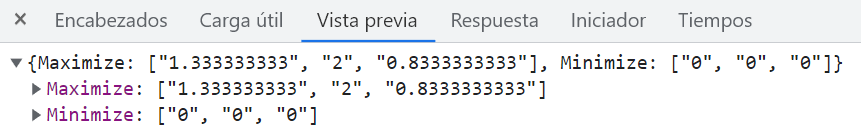
\includegraphics[width=1\textwidth]{img/respuestaJsonMax.PNG}
\caption{Respuesta JSON formado los arrays máximos y mínimos de una mezcla. }
\label{fig:respuestaJson}
\end{figure}

Por último, se muestra en la web los resultados de los cálculos junto con los botones de exportación de los datos de entrada y de la solución. 

\section{Problema subida API a Heroku}

Inicialmente se desarrolló el proyecto en dos códigos: una API que utilizaba la librería GLPK escrita en C y una parte front que se comunicaba con esta API mediante peticiones. Estos dos proyectos se desarrollaron por completo, funcionando ambos correctamente en un entorno local.

Uno de los requisitos del proyecto es que fuera una herramienta accesible, y que se desplegara como aplicación web. Por este motivo se seleccionaron Heroku para subir el proyecto back-end y Netlify para el proyecto front-end. Los códigos se consiguieron subir sin problemas. Pero en el caso de la API, necesitaba contar con la librería GLPK instalada en el servidor.  La librería GLPK usada en el entorno local no se consiguió instalara en un servidor web gratuito. 

Por este motivo, se tomó la decisión de cambiar el código front-end ya subido a producción, haciendo que el proyecto front-end en Angular, no necesitara el uso de la API. En este momento se realizó una búsqueda de librerías que pudieran ejecutarse en Typescript y resolvieran los mismos problemas que  el paquete GLPK. Las opciones finales fueron: \url{https://www.npmjs.com/package/glpk-ts} y \url{https://www.npmjs.com/package/glpk.js}. Finalmente, y ya que la lógica del código está desarrollada en Typescript se instaló y aprendió a utilizar \textbf{glpk-ts}. Este paquete es una interfaz de la misma librería GLPK \cite{glpk:package} que se usa desde módulos. 

Este cambio ha significado no realizar peticiones a la API, lo cual ha derivado en un desarrollo de estas funcionalidades en el proyecto front-end. 

\section{Internacionalización}

A través de la internacionalización se consigue realizar un proceso de expansión del software. Se ha diseñado la aplicación permitiendo intercambiar entre diferentes idiomas. Se proporcionan dos idiomas: Español e Inglés. Esto se permite desde una select en el menú superior que está siempre visible (figura \ref{fig:selectidiom}), cambiando este valor se lanza un evento que cambia una variable en el localStorage. Esta variable marca el fichero de traducciones a tomar por la aplicación. Los ficheros de traducciones se encuentran en la ruta \textbf{src/assets/i18n} y tienen extensión .json.

\begin{figure}[h!] 
\centering
    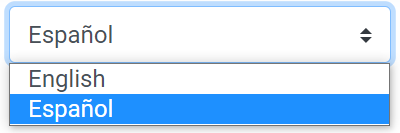
\includegraphics[width=0.4\textwidth]{img/selectIdiom.PNG}
\caption{Select de Idioma}
\label{fig:selectidiom}
\end{figure}

\newpage
Para realizar traducciones desde angular se hace uso del módulo Angular Translate, que mediante el pipe \textbf{translate} marca que ese texto tiene una traducción. En la ejecución de la aplicación se carga el fichero .json correspondiente a la variable \textbf{lang} en el localStorage. La estructura de estos archivos la podemos ver en la figura \ref{fig:en_json}: consiste en una cadena de texto (línea de código escrita en el fichero \emph{.html}), el símbolo \textbf{``:''} y una cadena de la traducción al idioma correspondiente.

\begin{figure}[h!] 
\centering
    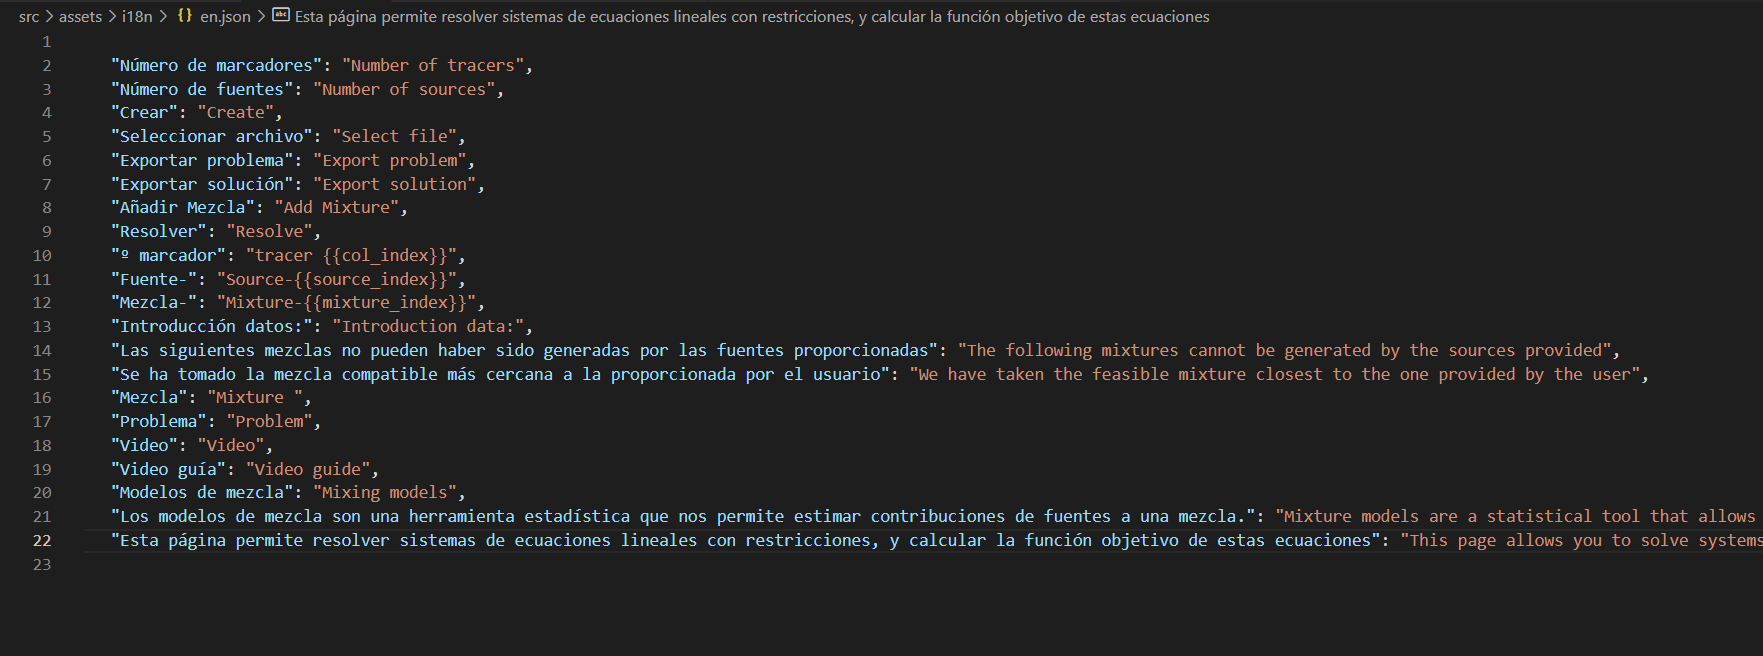
\includegraphics[width=1\textwidth]{img/en_json.PNG}
\caption{Archivo en.json}
\label{fig:en_json}
\end{figure}









\capitulo{6}{Trabajos relacionados}

%Este apartado sería parecido a un estado del arte de una tesis o tesina. En un trabajo final grado no parece obligada su presencia, aunque se puede dejar a juicio del tutor el incluir un pequeño resumen comentado de los trabajos y proyectos ya realizados en el campo del proyecto en curso. 

\section{Trabajos relacionados}
Este proyecto es el primer trabajo de fin de grado que implementa la resolución de problemas lineales para \emph{Mixing models} desde una web. Como objetivo de esta primera implementación se ha realizado el desarrollo una aplicación web híbrida.

\section{Proyectos similares}

\subsection{MixSIR} 

MixSIR fue el primer proyecto desarrollado por Jonathan W. Moore y Brice X. Semmens sobre Bayesian Mixing Models, que estimaba las proporciones de las fuentes en una mezcla, como herramienta de calculo para ecología.

En el artículo \cite{errorofMixSIR}, Andrew LLoyd Jackson, Richard Inger, Stuart Bearhop y Andrew C Parnell. Declaran un comportamiento erróneo de MixSIR. Mostrando ejemplos en los cuales MixSIR no identifica las proporciones dietéticas correctas más del 50\% de las veces.


\subsection{SIAR} 
SIAR es un paquete que utiliza cálculos estadísticos bayesianos principalmente orientado en la ecología sobre isótopos estables: calculando las contribuciones de las fuentes a una mezcla. Fue desarrollado por Parnell, A.C., Inger R., Bearhop, S. y Jackson, A.L. 2010 \cite{SIAR:Package}.

SIAR trabaja con unos términos de error residual por cada eje isotópico. Si los datos de las mezclas son muy variables respecto a las fuentes, se utiliza este término de error residual

\subsection{MixSIAR} 
MixSIAR es un paquete de R desarrollado por Brice Semmens, Brian Stock, Eric Ward, Agrew Parnell, Donald Phillips y Andrew Jackson. Es un proyecto colaborativo que incorpora los avances en Bayesian Mixing Models, combinando MixSIR y SIAR.

En el articulo \cite{analyzingMix2018} se describe su principal ventaja respecto a los desarrollos anteriores, permitiendo variar las proporciones de la mezcla y calcular mediante criterios de información el apoyo relativo.\\

Es importante comentar que ninguno de estos software se pueden utilizar vía web, ni tienen un diseño tan sencillo e intuitivo como el presentado en este proyecto.

\capitulo{7}{Conclusiones y Líneas de trabajo futuras}

En este capítulo incluiré mis conclusiones. Además, se citarán algunas posibles mejoras al proyecto o posibles líneas de desarrollo futuras.

\section{Conclusiones}

El tiempo que he dedicado al trabajo de fin de grado me ha permitido obtener muchas habilidades nuevas, especialmente sobre el desarrollo de aplicaciones web, aprendiendo los fundamentos de los principales lenguajes que se utilizan en estas aplicaciones. Se ha conseguido desarrollar una aplicación Single-page Application en Angular; por otra parte, se han utilizado librerías que resuelven problemas lineales utilizando una librería escrita en Typescript. Se aprendió a realizar peticiones desde una API a una web usando textos en JSON y apoyándome en Postman para comprobar el funcionamiento de las peticiones. También querría destacar el uso de estilos, principalmente por medio los Componentes que ofrece Bootstrap. Y también se ha aprendido sobre \LaTeX{}, que es un lenguaje de creación de documentos que se ha utilizado para realizar la documentación de este proyecto. Por último, he aplicado las metodologías ágiles para la planificación de este proceso.

\section{Posibles mejoras}
Algunas mejoras que consideramos interesantes ante posibles desarrollos futuros son:

\begin{itemize}
    \item \textbf{Mejorar la interfaz gráfica:} En la aplicación se han utilizado principalmente Componentes Bootstrap prediseñados, y se han reajustado algunos colores y posiciones, pero creemos que los estilos pueden aportar más calidad a la aplicación. Algunas nuevas mejoras serian hacer la aplicación más adaptativa (Responsive), añadir Spinner en los tiempos de carga, o aplicar un estilo más similar en toda la aplicación. 
    \item \textbf{App Android:} Creación de una App para móviles, añadiendo mejoras de diseño de interfaz y experiencia de usuario para los usuarios móviles, y diseño de un logo de la aplicación
    \item \textbf{Permita resolver otros problemas:} Añadir la resolución de otros problemas matemáticos que estén relacionados con problemas de Mixing Models.
    \item \textbf{Análisis de datos:} Añadir análisis de los resultados obtenidos, con sus correspondientes botones de exportación.
    %\item \textbf{Incluir manual de usuario: } En la aplicación de añadió un apartado con un vídeo a modo de guía de la aplicación, pero seria interesante añadir un manual de usuario que añada mas detalle sobre el funcionamiento de la aplicación.
\end{itemize}



\bibliographystyle{plain}
\bibliography{bibliografia}

\end{document}
